\subsection{Experimental Analysis}
%
In this section, we will test experimentally the setups discussed in section \ref{subsec:intro}.
%
%To obtain precise results form our setups, we will need to start by characterizing the devices that compose them.
%The output precision from our setups will depend on the correct characterization of the devices that compose them.
%Before any experiment, we will to need to characterize the devices that compose 
%The comparison between the theoretical and experimental results will require a high level of precision. therefore will need to correctly characterize the devices used on our setups.\\
This comparison between the theoretical and experimental results will require a high degree of precision from the devices used in these setups. Therefore, the correct characterization of these devices must be the starting point of this experimental phase.
One of the most fundamental components is the photodetector, which performs the signal's conversion from the optical domain into the electrical domain.
%
\subsubsection{Thorlalabs detector}
%
The detector used in the laboratory is the Thorlabs PDB 450C. This detector consists of two well-matched photodiodes and a transimpedance amplifier that generates an output voltage (RF OUTPUT) proportional to the difference between the photocurrents of the photodiodes.\\
Additionally, the unit has two monitor outputs (MONITOR+ and MONITOR-) to observe the optical input power level on each photodiode separately.
\cite{thorlabs}
%
\begin{figure}[H]
	\centering
	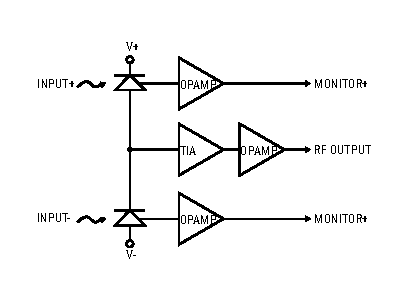
\includegraphics[width=10cm]{./sdf/optical_detection/figures/thorlabs-circuit.pdf}
	\caption{Functional block diagram of the PDB 450C Thorlabs detector \cite{thorlabs}}
	\label{fig:photodetector-circuit}
\end{figure}
%
\noindent
Figure \ref{fig:photodetector-circuit} shows a functional block diagram of the photodetector, in which the TIA (transimpedance amplifier) is an opamp-based current to voltage conversion amplifier.
In contrast to the photodiode's non-linear voltage response to incident light, it's current response is linear.
%\footnote{http://www.ti.com/lit/an/sboa035/sboa035.pdf, p.1}.
To take advantage of this linear response, the TIA is used to perform the conversion of the difference of currents between the two photodiodes into a voltage proportional to that same difference.\\
%\footnote{http://www.cypress.com/file/131966/download}.
%
\\
In section \ref{subsec:intro}, the relation between the input optical power and output current was established by a very simplified model of the photodetector.
%
%To make sense of the output current value, the photodetector model must be improved by characterizing it's parameters such as responsivity at various power levels and frequencies, bandwidth, amplification and noise levels.
%This model must be improved, in order that ... so, the various aspects of the photodiode such as (WHATEvA) 
%To improve the ("FIDELIDADE") of the detection process to our results??? will neeed to have full knowlege of the inner mechanisms of this device??? 
%To understad/contextualize the output of this system, we will need to understand the responde of this system to various settings ????
%To increase the precision of the system, we will need a more detailed model... 
To make sense of it's output, the photodetector model must be improved by characterizing it's parameters such as responsivity (at various power levels and frequencies), bandwidth, amplification and noise levels.
%
%The following tables and plots present values for a serie of parameters that can be readly obtained from the device's manual \cite{thorlabs}.\\
%From the devices's manual \cite{thorlabs}, a series of parameters can be readly obtained.
Various of those parameters can be readly extracted from the device's manual, which are presented in the following tables and plots.\\
%
%
%++ ITEMS DO PROF ++
%- responsividade do pin1 e do pin2
%- ganho do meu amplificar OPAMP
%- largura de banda
%- forma do filtro, espectro do filtro
%- ruído térmico, no braço superior, no braço intermédio e no braço inferior
%
%
\begin{table}[H]
	\centering
	\begin{tabulary}{1.0\textwidth}{|L|L|}
		\hline
		\textbf{Parameter}		& \textbf{Value}\\
		\hline
		Max Responsivity		& 1.0 A/W\\
		\hline
	\end{tabulary}
	\caption{Thorlabs PDB450C PIN parameters}
	\label{table:thorlabs}
\end{table}

\begin{table}[H]
	\centering
	\begin{tabulary}{1.0\textwidth}{|L|L|}
		\hline
		\textbf{Parameter}		& \textbf{Value}\\
		\hline
		Bandwidth				& 1 MHz\\
		\hline
		Voltage Gain			& 10 V/mW @ peak responsivity\\
		\hline
		Voltage Noise (RMS)		& <180 \textmu V (RMS)\\
		\hline
	\end{tabulary}
	\caption{Thorlabs PDB450C MONITOR +/- output parameters}
	\label{table:thorlabs}
\end{table}
%
%\noindent
%The manual also contains plots of the response in function of the input's signal frequency, for all the photodetector's outputs.
%Plot \ref{plot:freq-response-monitor} shows the response curves for the two MONITOR outputs. 
%
\begin{figure}[H]
	\centering
	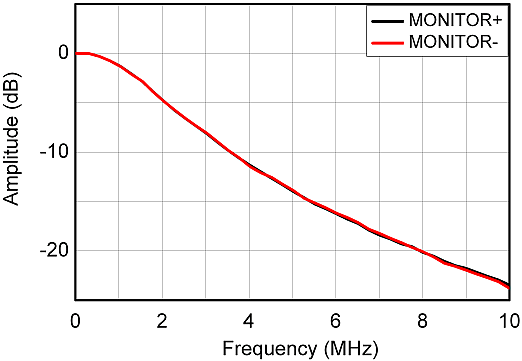
\includegraphics[width=8cm]{./sdf/optical_detection/figures/thorlabs-manual-gain-spec-monitor.png}
	\caption{MONITOR +/- output response with frequency. \cite{thorlabs}}
	\label{plot:freq-response-monitor}
\end{figure}
%
\noindent
The parameters of the RF OUTPUT have 5 values each, corresponding to the 5 gain settings of the TIA.
%
\begin{table}[H]
	\centering
	\begin{tabulary}{1.0\textwidth}{|l|cccccc|}
		\hline
		\textbf{Parameter}					& \multicolumn{6}{l|}{\textbf{Values}}\\
		\hline
		Bandwidth(-3dB)						& $150$  & $45$   & $4$    & $0.3$  & $0.1$  &MHz\\
		\hline
		Transimpedance Gain					& $10^3$ & $10^4$ & $10^5$ & $10^6$ & $10^7$ &V/A\\
		\hline
		Conversion Gain						& $10^3$ & $10^4$ & $10^5$ & $10^6$ & $10^7$ &V/W\\
		\hline
		Overall Output Voltage Noise (RMS)	& $0.50$ & $0.80$ & $1.0$  & $1.1$  & $2.0$  &mV\\
		\hline
	\end{tabulary}
	\caption{Thorlabs PDB450C RF OUTPUT parameters}
	\label{table:parameters-rf}
\end{table}
%
\begin{figure}[H]
	\centering
	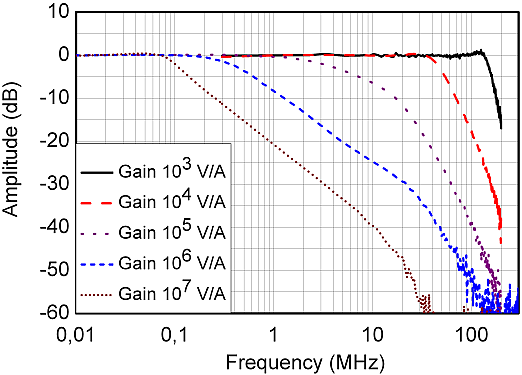
\includegraphics[width=8cm]{./sdf/optical_detection/figures/thorlabs-manual-gain-spec-rf.png}
	\caption{RF output response with frequency, for various gain values. \cite{thorlabs}}
	\label{plot:freq-response-rf}
\end{figure}
%
%
%\noindent
%{\em Gain response}\\
%The gain response is obtained by fixing an frequency $\omega_0$ and generating optical signals with various amplitudes $A_i$, such as $V = A_i \sin \left( \omega_0 t \right)$ and reading the output voltage amplitude.
%\footnote{REF?}\\
%\\
%{\em Frequency response/Bandwidth}\\
%The frequency response is obtained by fixing an amplitude $A_0$ and generating  optical signals with various frequencies $\omega_i$, such as $V = A_0 \sin \left( \omega_i t \right)$ and reading the output voltage amplitude.
%\footnote{REF?}
%%
%%
\subsubsection{Data analysis}
%
For each configuration of amplitude and frequency of the input signal, the photodetector output voltage is collected by the Digital Oscilloscope during a time interval and saved in a data file. The data consists on a sequence of pulses and it's analysis will be focused on the samples with equal phase. The steps will be the following
%
\begin{enumerate}
\item For each phase value, the average and variance of the samples with the same phase is calculated;
\item The representative amplitude and variance for the present configuration will be the obtained from the middle of the maximum plateau.
\end{enumerate}
%
%
%
%
To confirm the theoretical results obtained in section \ref{subsec:intro}, two experimental setups will be created. In the first experiement, we will study quantum noise in the single homodyne detection. The experimental setup will be based on the paper \cite{chi2011balanced}. In the second experiment, we will study quantum noise in the double homodyne detection setup, which will be basically an extension of the single homodyne detection setup.\\
\\
\subsubsection{Single homodyne detection}
%
To keep the experiment simple and avoid extra sources of noise, we will avoid using black boxes wich have complicated inner workings, having a preference in using simple components, as shown in fig. \ref{fig:experimental_homodyne_setup}:
\\
\begin{figure}[H]
	\centering
	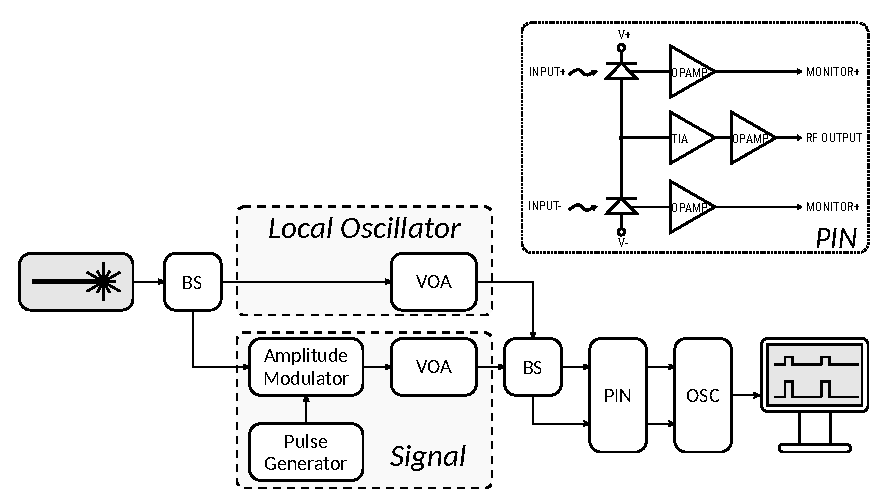
\includegraphics{./sdf/optical_detection/figures/scheme_experimental.pdf}
	\caption{Experimental setup}
	\label{fig:experimental_homodyne_setup}
\end{figure}
%
%
Material list
\begin{table}[H]
	\centering
	\begin{tabulary}{1.0\textwidth}{|L|L|l|}
		\hline
		\textbf{Device}		& \textbf{Description}\\
		\hline
		Local Oscillator	& Yenista OSICS Band C/AG\\
		\hline
		BS					& Beam Splitter\\
		\hline
		Pulse Generator		& HP 8116A Pulse Generator\\
		\hline
		Amplitude Modulator	& Mach Zehnder SDL OC 48\\
		\hline
		VOA					& Eigenlicht Power Meter 420\\
		\hline
		VOA					& Thorlabs VOA 45-APC\\
		\hline
		PIN					& Thorlabs PDB 450C\\
		\hline
		ADC					& Picoscope 6403D\\
		\hline
	\end{tabulary}
\end{table}
%
A single laser is splitted and used as the source for the signal (S) and the local oscillator (LO). The signal beam is pulsed and highly attenuated. The local oscillator is also attenuaded, but not pulsed. The signal and local oscillator interfere in a Beam Splitter originating two beams which are then converted to voltages in the PIN. These voltages are read in the Digital Oscilator (OSC) and collect in the computer. In the post processing phase, the quantum noise is measured by applying a difference between the two beams and measuring it's variance.
\\
The second stage of the experiment will be very similar to the first one, in which the signal and local oscillator branches will be divided. One of the new branches of the local oscilator will suffer a phase delay of $\pi/2$, in order to measure the quadrature component of the incoming signal.\\
%%
%%

\subsection{Comparative analysis}
%
%WARNING -- OLD DATA --\\
%
Given the theoretical, simulated and experimental frameworks, we will now compare the results obtained by each of them.
\\
%
\begin{figure}[H]
	\begin{subfigure}{.5\textwidth}
		\centering
		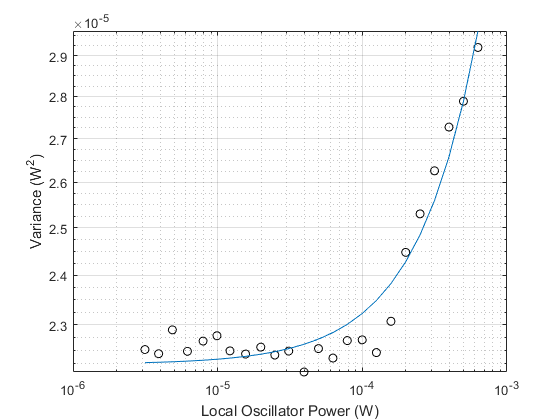
\includegraphics[width=.8\linewidth]{./sdf/optical_detection/figures/noise_exp_channel1.png}
		\caption{$X$ quadrature}
		\label{fig:noise-exp-1}
	\end{subfigure}%
	\begin{subfigure}{.5\textwidth}
		\centering
		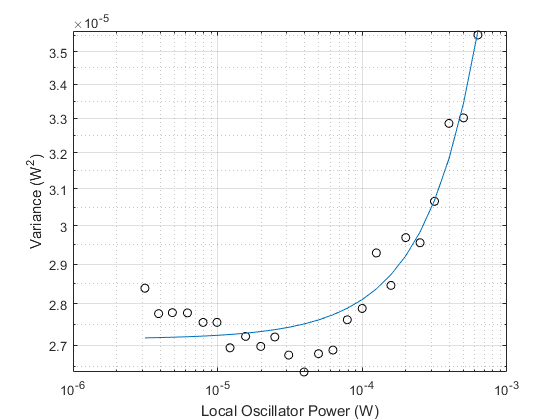
\includegraphics[width=.8\linewidth]{./sdf/optical_detection/figures/noise_exp_channel3.png}
		\caption{$Y$ quadrature}
		\label{fig:noise-exp-3}
	\end{subfigure}
	\captionsetup{justification=centering}
	\caption{Noise variance dependency with local oscilator power for two different quadratures. Experimental vs fitted data.}
\end{figure}
%
Figures $\ref{fig:noise-exp-1}$ and $\ref{fig:noise-exp-3}$ show measurements of total noise for two different quadratures. For low power of LO, the noise variance flutuates around a constant value. For high power of LO, $(P_{LO}>10^{-4}W)$, the variance of noise shows an increasing trend roughly proportional to $P_{LO}^2$. The polynomial fittings confirm this trend, showing a degree 2 coefficient much larger than the degree 1 coefficient
%
\begin{equation}
\textrm{Var}_X = 2.22 \!\! \times \!\! 10^{-5} + 9.6 \!\! \times \!\! 10^{-3} P_{LO} + 3.40 P_{LO}^2
\end{equation}
\begin{equation}
\textrm{Var}_Y = 2.71 \!\! \times \!\! 10^{-5} + 8.9 \!\! \times \!\! 10^{-3} P_{LO} + 7.25 P_{LO}^2
\end{equation}
%
The expected growth should be proportional to $P_{LO}$, but the RIN noise, originated by the electric apparatus, which grows quadratically with the power, is dominating the noise amplitude for large $P_{LO}$.\\
We see that both the simulation and experimental data display a similar behaviour, but the quadratic growth of noise for large $P_{LO}$ was not predicted in the simulations.\\ 
